\documentclass[./main.tex]{subfiles}

\begin{document}

In this section, the order for the integration of the components will be
described. This is useful for the planning of the implementation. If many
components are implemented simultaneously, the order for the integration shown
in this section avoids wasting time due to dependencies not considered.

\subsubsection{Integration of the application server}

The components inside the application server are quite independent. They can be
developed in any order, except for \textbf{Router}, that must be developed as
last since it uses the interfaces of the other components. The figure
\ref{fig:integration_router} shows the diagram for the integration.

\begin{figure}[H]
\centering
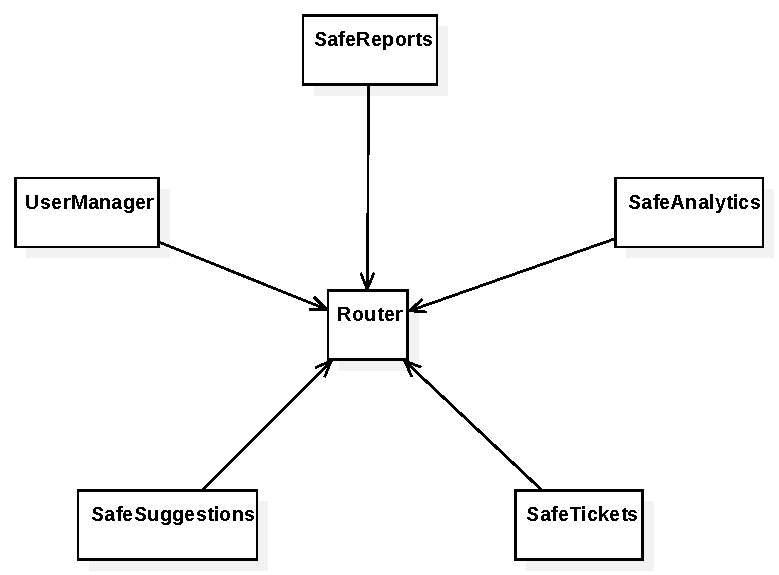
\includegraphics[width=\textwidth]{resources/integration_diagrams/integration_router}
\caption{ApplicationServer integration}
\label{fig:integration_router}
\end{figure}

\subsubsection{Integration of the internal components}

The only internal components that consists of more than one sub-element are
\textbf{SafeSuggestion} and \textbf{SafeReports}. The first one does not need
any diagram since the two sub-components are independent one from another. The
second one must follow the integration order of the diagram in figure
\ref{fig:integration_report_manager}.

\begin{figure}[H]
\centering

\includegraphics[width=\textwidth]{resources/integration_diagrams/integration_report_manager}
\caption{ReportManager integration}
\label{fig:integration_report_manager}
\end{figure}

\subsubsection{Integration with external components}

The diagram in figure \ref{fig:integration_client_server} shows the order for
the integration of the application with the external components. Since the
external component are not developed by SafeStreets itself, they are considered
as pre-existing.

\begin{figure}[H]
\centering
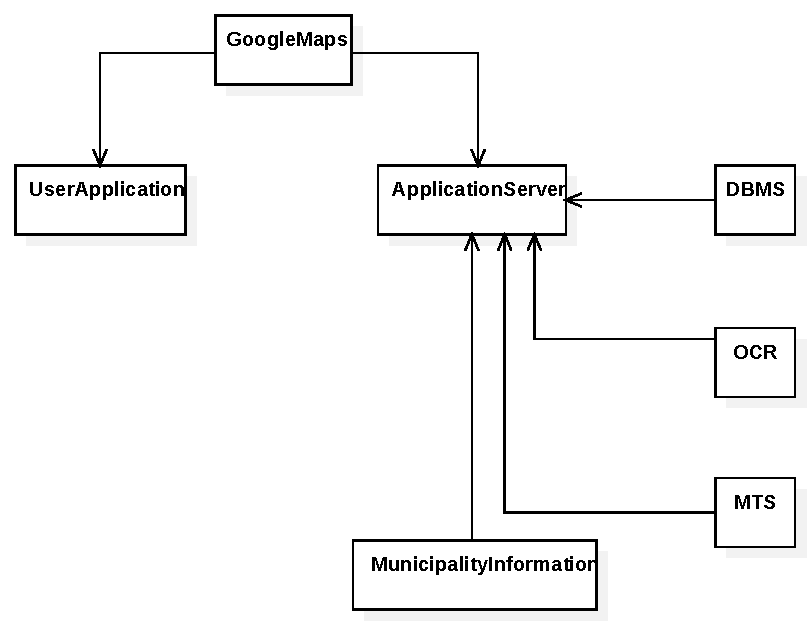
\includegraphics[width=\textwidth]{resources/integration_diagrams/integration_client_server}
\caption{External components integration}
\label{fig:integration_client_server}
\end{figure}

\end{document}